\documentclass[UTF8,fontset=none,a4paper]{ctexart}
\usepackage[a4paper,margin=2.5cm]{geometry}
\setCJKmainfont{NotoSerifCJKsc-Regular.otf}[Path=fonts/,BoldFont=NotoSerifCJKsc-Bold.otf]
\setCJKsansfont{NotoSansCJKsc-Regular.otf}[Path=fonts/,BoldFont=NotoSansCJKsc-Bold.otf]
\setCJKmonofont{NotoSansCJKsc-Regular.otf}[Path=fonts/]
\usepackage{amsmath,amssymb,graphicx,booktabs,array}
\usepackage[authoryear,round]{natbib}
\usepackage{url}
\usepackage[hidelinks]{hyperref}
\def\UrlBreaks{\do\/\do-\do.}
\bibliographystyle{plainnat}
\setcitestyle{authoryear,round,semicolon}
\ctexset{section/format=\Large\bfseries\raggedright}
\pagestyle{plain}
\title{所知多于所言：极简身体中的冻结语言模型\\[0.5em]\large Knowing More Than It Can Say: Frozen Language Models in Minimal Bodies\\[0.8em]\normalsize 本文为英文预印本的中文译本，由 AI 辅助翻译。如有出入，以英文原文为准。}
\author{Egor Grigorev\\ ORCID: \href{https://orcid.org/0009-0000-2725-5466}{0009-0000-2725-5466}}
\date{预印本，2026 年 10 月}
\begin{document}
\maketitle
\begin{abstract}
冻结的预训练语言模型越来越多地被用作具身智能体的组成部分，但在这类场景中预训练究竟贡献了什么，以及模型内部表征的信息有多少能够通过其输出获得，目前尚不清楚。我们在一个极简的二维觅食环境中研究这一问题：智能体的身体事件（body events）以一段简短的离散标记序列呈现给冻结语言模型（frozen language model），并将每个预训练（pretrained）模型与具有相同架构、随机权重（random weights）且嵌入范数匹配的模型进行比较。在三个模型家族（Pythia 160M--6.9B, Qwen2.5-1.5B, OLMo-2-1B）上，我们发现：(i) 在预训练有帮助的情形下，其优势来自序列处理机制而非词义------任意事件词（event words）的效果与有意义的事件词相当或更好，并且在一个家族（Qwen2.5）中，优势只在使用任意词时出现；(ii) 一个在上下文中从未被明确陈述的回合（episode）隐变量（latent variable）可以从隐藏状态中被线性解码（linearly decodable），AUC 为 0.93--0.99，但模型对直接提问的回答只能以 AUC 0.61--0.64 恢复它，而且在 Pythia 中，来自其他回合的上下文示例并不能缩小这一差距；(iii) 一个词的含义（食物与有害之分）在该词的位置上完整存在，但到达最终位置（回合层面的读出会在此处使用它）时至多只是微弱的（0.97--1.00 对 0.51--0.62）；(iv) 当词义与上下文中的经验相冲突时，经验在回答中留下统计上可靠的痕迹，但明显弱于词义效应（为其 4--28\%），且回答基本不变。所有主要分析均以带时间戳的提交进行了预注册（preregistration），使用精确置换检验（permutation test）或自助法（bootstrap）并进行 Holm 校正（Holm correction），并包含对混杂因素（confound）的对照------这些混杂因素在项目进行过程中曾误导或本可能误导我们的结论，例如幸存者偏差（survivorship）所造成的频率线索。综合来看，结果表明：处于这一状态的冻结语言模型对其具身情境的表征（representation）远多于它们所能表达（expression）的内容，瓶颈在于传递（routing）与表达，而不在于表征。
\end{abstract}

\section{引言}

语言模型越来越多地被提议用作监测和控制物理过程的系统组件：作为具身智能体的规划器 \citep{ahn2022,huang2022}，作为由预训练（pretrained）权重初始化的策略 \citep{li2022,reid2022}，以及在工业场景中作为诊断层，用于解读传感器数据流并向人类操作员解释异常 \citep{dave2024,li2026,liu2025}。在发电等安全关键的基础设施中，这类组件的价值与其说取决于解释是否流畅，不如说取决于它所说的内容是否反映了它实际登记到的信息。一个口头报告（report）与其内部状态不一致的诊断层是一种风险：操作员依据报告行事，而不是依据状态。

这个问题对我们而言并非假设。作者运营燃气发动机发电设施，并开发 KONTUR------一个面向发电机组的仅观测（observation-only）监测（monitoring）系统，其中包含一个为技术人员生成解释的机器学习诊断层。在该系统中，没有任何自动决策作用于设备；每一项操作都由操作员执行。要判断语言模型能否在这样的角色中被信任，以及应当读取它的什么------输出还是内部状态------就需要知道模型关于一个物理情境所表征的内容中，有多少真正到达了它的输出。

我们在一个刻意极简的设置中研究这一问题，其目的是分离机制，而不是追求真实。一个模拟智能体在二维觅食环境中经历离散的身体事件（body events）------它吃了哪一种类（kind）的物品，以及能量是上升还是下降------这些事件以简短的标记序列呈现给一个冻结的预训练语言模型。回合（episode）的一个隐变量（latent variable），即当前哪一种类的物品是食物，在上下文中从未被陈述；它只能从事件的组合中推断出来。这使我们能够提出三个明确的问题：预训练对处理这类事件流贡献了什么，隐变量是否在模型的隐藏状态中被表征（representation），以及当被直接询问时模型能否报告它。

在三个模型家族上，我们发现了表征与报告之间一致的分离。隐变量几乎可以从隐藏状态中被完美地线性解码（linearly decodable），而模型自身的回答只能微弱地恢复它；一个词的含义在该词的位置上完整存在，但几乎没有到达回合层面读出会使用它的位置；当词义与上下文中的经验相冲突时，经验在回答中留下可测量但很小的痕迹，并且基本上不改变回答。在预训练有帮助的情形下，它所贡献的是一种序列处理机制，这种机制在任意符号上的效果至少与在有意义的符号上一样好，而不是词的含义；在 Qwen2.5 中，优势只在使用任意符号时出现。针对事实知识的探针（probe）研究曾报告过模型所编码的内容与其所表达的内容之间的相关差距 \citep{orgad2024,gekhman2025,burns2022,azaria2023}。与以往关于隐藏事实知识的研究不同，我们的目标变量并不存储在预训练参数中：它是根据智能体当前的经验在线构建的。

我们的贡献如下：
\begin{enumerate}
\item 一个受控设置，其中情境隐变量必须从上下文中的身体事件推断出来，并且每一项比较都配有相同架构的随机权重（random weights）对照；
\item 对表征与报告之间差距的测量------针对回合隐变量、针对词义以及针对词义与经验的对抗------在 Pythia、Qwen2.5 和 OLMo-2 上得到复现，我们将其解释为由表征、传递（routing）和表达（expression）构成的三层图景；
\item 一套带有时间戳提交的预注册（preregistration）方法以及所有尝试的登记表，其中包括一组有记录的混杂因素（confound），它们在项目进行过程中曾误导或本可能误导我们的结论------其中包括幸存者偏差（survivorship）造成的频率线索，以及经由智能体自身闭环（closed-loop）行为的捷径------以及捕捉到它们的对照（第 4 节）。
\end{enumerate}

我们并不声称这些发现能够直接迁移到已部署的监测系统，后者使用更大的模型、更丰富的输入，并且往往具有经过训练的输出通道。我们得出的实际含义要窄得多：在语言模型的输出被当作关于物理系统的证据的角色中，其输出与内部状态之间的对应关系应当被测量，而不是被假定。


\section{设置}

\subsection{环境}

所有分析都使用一个极简的二维觅食世界 flip-2。一个回合（episode）持续 100 步，在单位正方形内进行，两个种类（kind）A 和 B 各有两个物品。在每个回合中，一个种类是食物（+0.35 能量），另一个是毒物（$-$0.20）。哪一种类是食物------即回合符号（episode sign，哪类物品为食物）------在开始时由抛硬币决定，在 30 到 69 之间的随机一步翻转一次，并且从不被直接观测。身体只报告事件：这一步吃了哪一种类（如果有的话），以及能量是上升、下降还是不变。没有食物时能量会向下漂移，因此身体有其自身的时间。对于本文报告的分析，轨迹由盲策略（blind policy）生成，即一种朝最近物品（不论种类）移动的反射。因此模型读取的是并非由它塑造的经验，经由行为的闭环（closed-loop）捷径被排除。

\subsection{接口}

\textbf{事件词（event words）。} 每一步写成两个标记：所吃的种类（`` A''、`` B'' 或 `` none''）和结果（`` up''、`` down'' 或 `` same''）。窗口（window）之前有一个起始标记（start token），窗口覆盖最近 32 步。回合符号在窗口中的任何地方都没有被陈述。它只能通过将一个种类与其后的结果绑定（binding）来推断。在较早的一种接口中，连续传感器特征经由固定的随机投影进入嵌入空间，此时预训练（pretrained）模型并不优于随机模型（第 3.1 节）。对于任意词对照（第 3.2 节），六个事件词被替换为无关的单标记词（例如 `` cat''、`` table''、`` stone'' / `` river''、`` chair''、`` door''）。

\textbf{问题。} 为了读取模型的回答，在窗口后附加一个问题（`` Food:''、`` Safe to eat:''、`` Good kind:''），回答是最后位置上 `` A'' 与 `` B'' 之间的 logit 差值（logit difference）。

\textbf{带有含义的种类词。} 为了检验词义（第 3.4 节），两个种类符号被替换为含义为食物（例如 apple、bread）或有害（例如 mold、glass）的词。这些词来自各含 30 个单标记词的词池，直接表示可食性的词被排除。

\textbf{合成窗口（synthetic windows）。} 为了在没有任何频率线索的情况下分离词义与经验（第 3.5 节），我们构造由短句组成的窗口（``I ate w. Energy went up.'' / ``\ldots{} went down.'' / ``Nothing happened.''）。
\begin{itemize}
\item 每个窗口包含 n $\in$ \{2, 4, 6\} 个事件，每个种类恰好 n/2 个。第一个和最后一个事件的种类，以及用于评分的参照种类，在每个单元内都是平衡的。
\item 频率参照、最后提及参照和首次提及参照在这些窗口上的得分都恰好为 0.5。一个读取种类--结果绑定的贝叶斯读者得分为 1.0。
\item 对照保留词、位置和顺序，并在事件之间置换结果，使绑定不含信息。
\item 共使用十组，每组 648 个窗口。
\end{itemize}

\subsection{模型与对照}

\begin{itemize}
\item \textbf{模型：} Pythia 160M--6.9B、Qwen2.5-1.5B 和 OLMo-2-1B，全部冻结，以 fp32 运行并禁用 TF32。
\item \textbf{随机权重（random weights）对照。} 每个预训练模型都与具有随机权重的相同架构进行比较；其输入嵌入被重新缩放到预训练嵌入的平均行范数。随机网络对每一组重新设定种子，词义探针（第 3.4 节）除外，它对每个模型使用一个随机网络。
\item \textbf{分词器迁移。} 在跨家族复现中，每个协议在没有其他改动的情况下被迁移：
\begin{itemize}
\item 起始标记是每个模型的文档结束标记 ``<|endoftext|>''。在 Pythia 和 OLMo-2 中它是 BOS 标记；Qwen2.5 默认没有 BOS；
\item 在全部三种分词器中，每个词都是带前导空格的单个标记，因此不需要任何替换；
\item 所有输入都通过解码进行了核验；
\item 经由迁移后代码运行的 Pythia-1B 复现了原始数值（例如词义探针为 0.983 / 0.526 / 1.000）。
\end{itemize}
\end{itemize}

\subsection{测量}

\textbf{探针（probe）。} 探针是作用于最后一层隐藏状态的 L2 正则化逻辑回归。特征在每一折的训练部分上标准化，正则化强度通过内部验证选择。当探针在具有相同符号的新回合上测试时，各折按回合分组（第 3.1--3.3 节）。当探针必须泛化到新词时，各折按词分组，因此测试词在训练中从未出现（第 3.4 节）。符号探针报告平衡准确率（balanced accuracy）；其他探针报告 AUC。

\textbf{回答。} 回答是问题之后两个回答标记之间的 logit 差值，以相对于真实符号的 AUC 评分，或者以平均 logit 偏移评分（第 3.5 节）。读取 logit 而不是采样文本，依据的是这样一个论点：基于提示的判断可能低估模型所编码的内容 \citep{hu2023}。

\subsection{统计与预注册}

\begin{itemize}
\item \textbf{主要检验。} 在 10 组上进行精确配对符号翻转置换检验（permutation test）（1,024 次置换）；在方向已预注册的情况下为单侧检验，在最早的分析中为双侧检验。
\item \textbf{词义探针。} 它使用单侧自助法（bootstrap）（10,000 次重抽样）。
\item \textbf{区间。} 当探针泛化到新词时，区间是按词的聚类自助法（cluster bootstrap），而不是按回合。其他区间是各组上的 95\% t 区间。
\item \textbf{多重性。} 在每个预注册的检验族内进行 Holm 校正（Holm correction）。
\item \textbf{预注册（preregistration）。} 每一项主要分析都在计算任何数据之前的一次提交中进行了预注册，所有结果及其解释都事先写明。每一次尝试，包括被放弃的环境变体，都列在登记表中。在看到数据之后添加的分析被标注为事后分析（post hoc）。
\end{itemize}

\section{结果}

\subsection{接口决定预训练是否有帮助}
\begin{figure}[t]\centering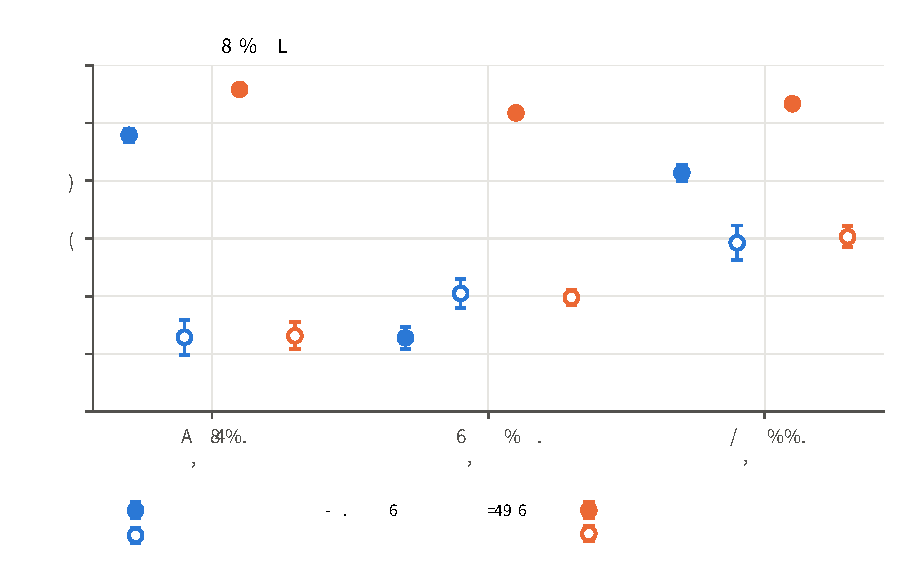
\includegraphics[width=\linewidth]{figures/F2_words_vs_random.pdf}
\caption{\textbf{有意义的事件词与任意事件词对比。}窗口最终位置上回合符号线性探针的平衡准确率（balanced accuracy），使用有意义的事件词（A, B, none / up, down, same；蓝色）或任意单标记词（两组词的平均；橙色）；实心：预训练，空心：随机权重。每个模型 10 组 $\times$ 200 个回合；各组的均值和 95\% t 区间。数据：A28（A3 和 A4 的协议）。}\label{fig:words}\end{figure}

\textbf{连续投影器。} 当身体状态经由连续投影器进入时，预训练（pretrained）的 Pythia 并不优于随机权重（random weights）：在 160M 时它显著更差（$-$0.053，Holm p = 0.012）。

\textbf{起始标记与事件词。} 加入起始标记（start token）消除了大部分差距：在 160M 时，预训练与随机之间的差值从 $-$0.054 变为 $-$0.008，改善了 +0.047（Holm p = 0.004）。将事件写成词使预训练模型首次获得优势：相对于投影器接口，预训练与随机之间的差距改善了 +0.191（Holm p = 0.004），符号探针（probe）的平衡准确率（balanced accuracy）为 0.950 对 0.813（160M），描述性地为 0.951 对 0.856（410M）。

\textbf{复现。} 这一优势在 OLMo-2-1B 上得到复现（0.963 对 0.938，Holm p = 0.006），并在 Pythia-1B 上描述性地复现（0.976 对 0.906）。在使用这些事件词（event words）时，它在 Qwen2.5-1.5B 上\textbf{没有}复现：0.906 对 0.921，预训练模型在 9 组（共 10 组）中更低。使用任意事件词时，预训练的 Qwen2.5 再次明显领先（0.983 对 0.920）（图~\ref{fig:words}）。我们没有探究为什么类似字母的符号对 Qwen2.5 不利。因此，``事件词使预训练能够发挥作用''这一论断成立，但附带关于模型家族和符号集的保留。

\subsection{是机制，而非含义}

\textbf{Pythia-160M。} 如果优势来自事件词的含义，那么无关的词应当消除它。事实并非如此。在 160M 时，任意词比有意义的词好 0.016（Holm p = 0.004），并且使用任意词的预训练模型比随机权重高 0.156（Holm p = 0.004）。将预训练模型的六个事件嵌入替换为相同范数的随机向量，描述性地仍得到 0.984。对某一组任意词的表面偏好后来被追溯为标记上的运气，因此我们将结果表述为``不更差''而不是``更好''。

\textbf{复现。} 在三个家族中，任意词都不劣于有意义的词并高于随机权重（Holm p = 0.006，见于 Qwen2.5 和 OLMo-2，针对要求两者同时成立的预注册检验；Pythia-1B 为描述性结果）。相对于有意义的词，差值为 +0.016（Pythia-1B）、+0.078（Qwen2.5）和 +0.024（OLMo-2）（图~\ref{fig:words}）。

预训练在这里所贡献的是作用于离散符号的序列处理机制，而不是符号的含义。这与以下发现相呼应：无论输入是否为自然语言，语言模型初始化都有助于决策 \citep{li2022}；随机 Transformer 已经具备某些算法能力 \citep{zhong2024}。

\subsection{被表征，但未被报告}
\begin{figure}[t]\centering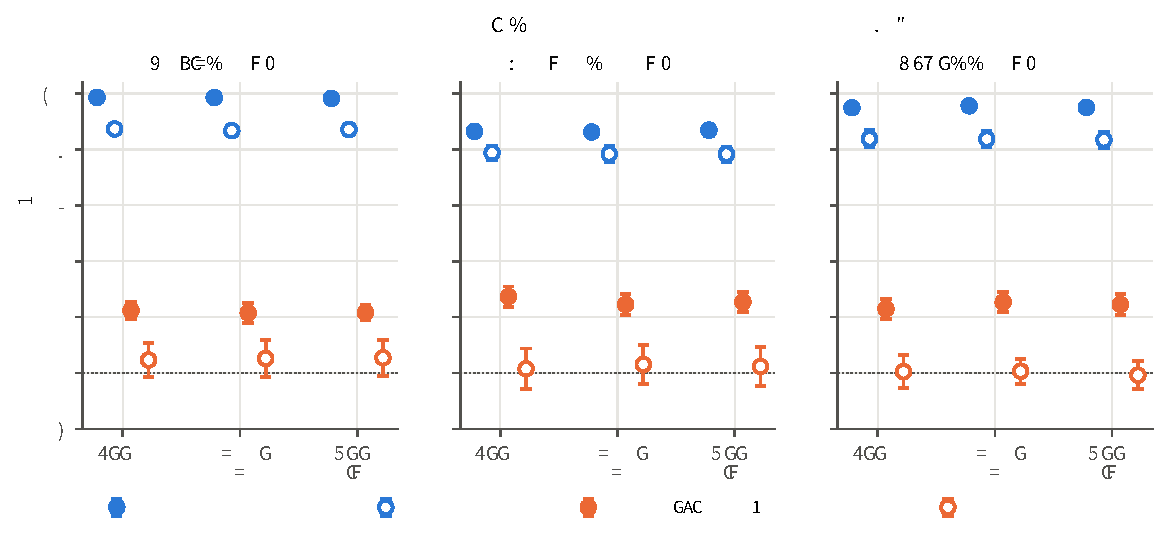
\includegraphics[width=\linewidth]{figures/F1_probe_vs_answer.pdf}
\caption{\textbf{隐含回合符号的探针与回答对比。}针对回合符号（episode sign）的 AUC：问题位置上的线性探针（probe）（蓝色），以及模型的回答，即 logit 差值（logit difference）`` A'' $-$ `` B''（橙色），对应三个零样本问题。实心标记：预训练（pretrained）；空心：相同架构、随机权重（random weights）且嵌入范数匹配。flip-2，32 步事件词窗口；每个模型 10 组 $\times$ 100 个回合；各组的均值和 95\% t 区间。数据：A28（A22 的协议）。}\label{fig:probe}\end{figure}

\textbf{表征（representation）。} 回合符号（episode sign）在窗口中从未被陈述，但问题位置上的线性探针以 AUC 0.993、0.932 和 0.975 将其解码（Pythia-1B、Qwen2.5、OLMo-2；第一个问题）。

\textbf{回答。} 当被直接询问时，同样的模型回答得差得多：在三个问题上 AUC 为 0.607--0.612、0.623--0.637 和 0.615--0.627。这重复了最初的 Pythia 结果（零样本 AUC 0.61，而探针为 0.98--0.99）。

\textbf{预注册标准。} 回答超出随机水平的部分至多为探针的一半，即 (AUC\_answer $-$ 0.5) $\le$ 0.5 $\cdot$ (AUC\_probe $-$ 0.5)。它在所有三个家族的所有三个问题上都成立（图~\ref{fig:probe}）。探针是在读取回答的同一位置的隐藏状态上训练的；因此它是从该状态出发的一座经过训练的线性桥梁。所以探针与回答之间的差距指向从这一状态到回答标记的映射，而不是指向该位置上信息的缺失。

\textbf{有两项观察对这一图景加以限定。}
\begin{itemize}
\item 随机权重网络同样支持很高的探针结果（0.892--0.937），而它们的回答停留在随机水平（0.50--0.53）。描述性地看，预训练对回答通道（answer channel）的增益（+0.09 至 +0.13 AUC）大于对探针的增益（+0.04 至 +0.06）。我们没有检验这一差异。
\item 仅在 Pythia 中，上下文示例没有缩小这一差距。来自同一回合的示例只是被复制：少样本 AUC 0.974 与``重复最后一个示例的回答''对照的 0.975 相当。来自其他回合的示例给出随机水平：AUC 0.505（160M）、0.469（1B），并不高于随机权重或复制对照（Holm p $\ge$ 0.6）。A23 仅在 Pythia 上运行。
\end{itemize}

这一模式------内部状态所编码的内容多于模型输出所揭示的内容------已有针对事实知识和真实性的报告 \citep{orgad2024,gekhman2025,azaria2023}；而在这里，它涉及一个只存在于智能体近期身体经验中的变量。

\subsection{词义停留在局部}
\begin{figure}[t]\centering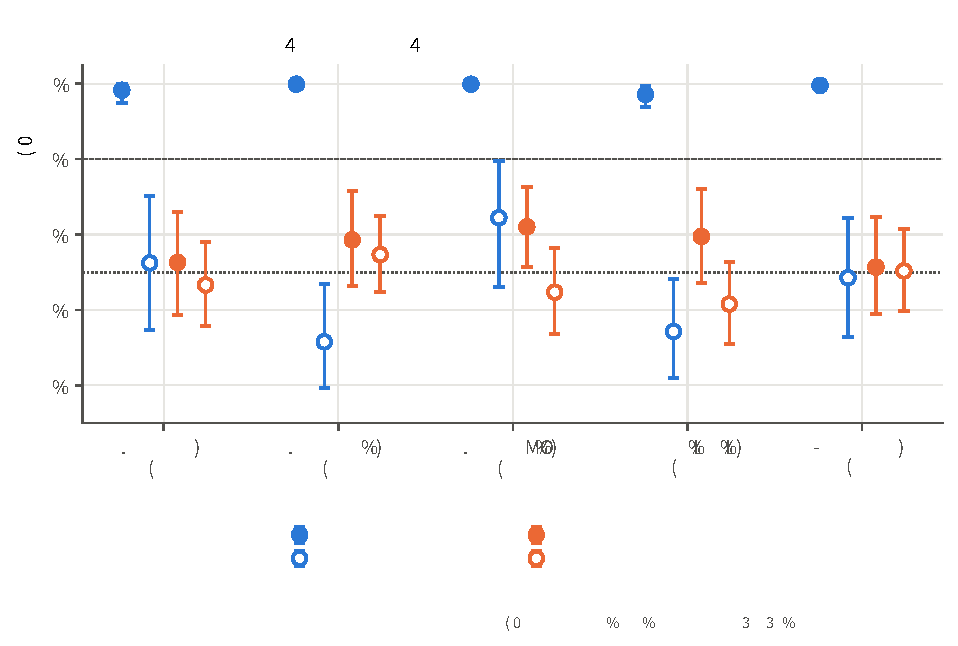
\includegraphics[width=\linewidth]{figures/F3_meaning_by_position.pdf}
\caption{\textbf{按位置的词义。}针对``种类词表示食物''的线性探针的 AUC，在训练中从未见过的词上测试，分别在种类词自身的位置（蓝色）和窗口最终位置（橙色）读取；实心：预训练，空心：随机权重。Pythia 1B / 2.8B / 6.9B（来自 A24）与 Qwen2.5-1.5B / OLMo-2-1B（来自 A28）在不同的 RTX 5090 实例上计算；这两组之间的比较是描述性的。200 个回合，$\approx$56 个不同的测试词；按词的 95\% 聚类自助法（cluster bootstrap）区间。随机权重：每个模型一个网络；在独立随机网络之间，AUC 分布在 $\approx$0.36--0.63（模拟）。虚线：预注册阈值 0.8。}\label{fig:meaning}\end{figure}

\textbf{语言中的词义。} 模型知道哪些词表示食物。在中性句子（``The apple.''）中，作用于该词隐藏状态、在留出词上测试的探针，以 AUC 1.000、1.000 和 0.999（Pythia 1B、2.8B 和 6.9B）以及 1.000（Qwen2.5 和 OLMo-2）区分食物词与有害词。直接词（edible 与 poison）作为该方法的阳性对照（1.000 / 0.967 / 0.967；0.900；0.967）。

\textbf{事件窗口中的词义。} 当同样的词作为种类（kind）符号出现时，探针------在训练中从未见过的词上测试------在种类词自身的位置上读出其含义：0.983--0.999（Pythia）、0.972（Qwen2.5）和 0.996（OLMo-2）。在最终位置（回合层面的读出会在这里查看），它至多达到 0.53--0.62：0.526 / 0.586 / 0.620（Pythia 1B / 2.8B / 6.9B），0.595（Qwen2.5）和 0.514（OLMo-2）（图~\ref{fig:meaning}）。

\textbf{区间。} 由于探针泛化到新词，区间是对 $\sim$56 个测试词的聚类自助法（cluster bootstrap）。对于最终位置上的 Pythia-6.9B，这给出 0.620 [0.51, 0.73]，而随机权重为 0.447 [0.33, 0.56]。因此我们并不声称 6.9B 向最终位置传递的词义多于随机网络。我们只声称没有任何模型达到预注册阈值 0.8。

\textbf{低于 0.5 的随机权重数值。} 这些数值（例如 0.315，Pythia-2.8B）并不是按词分组划分造成的假象。在随机词向量上对同一程序进行模拟，得到的均值为 0.495，独立随机网络分布在 0.36--0.63 之间。

因此，一个词的含义存在于该词所在之处，但并没有被传递（routing）到概括回合的位置。这与关于模型如何在上下文中将属性绑定到实体的研究一致 \citep{feng2023}。

\subsection{词义对抗经验：不改变回答的微弱痕迹}
\begin{figure}[t]\centering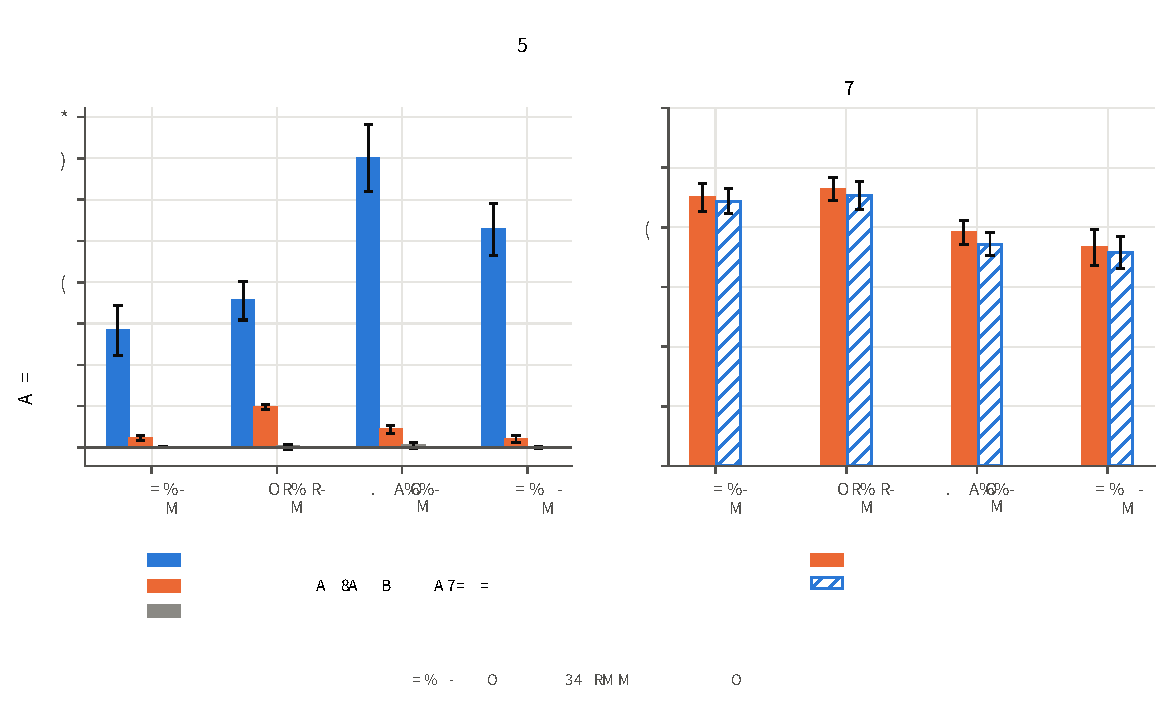
\includegraphics[width=\linewidth]{figures/F4_synthetic_binding.pdf}
\caption{\textbf{合成窗口中的词义对抗经验。}(a) 在冲突窗口上（种类词的含义与结果相矛盾）：词义效应，即结果被置换的同一批窗口上的 |d|（蓝色）；向经验的偏移，d(outcomes) $-$ d(permuted)（橙色）；随机权重的同一偏移（灰色）；d 是真实食物词与毒物词之间的 logit 差值。(b) 回答偏向经验的冲突窗口比例，有结果（橙色）与结果被置换（斜线填充）。句子接口，每个窗口 2--6 个事件，10 组 $\times$ 648 个窗口；各组的均值和 95\% t 区间。Pythia-1B、Qwen2.5-1.5B、OLMo-2-1B：A28（同一实例）；Pythia-6.9B：A27（另一个实例）。}\label{fig:synth}\end{figure}

\textbf{为什么使用合成窗口（事后分析，Pythia）。} 第一项检验使用了模拟身体（Pythia 1B--6.9B）。
\begin{itemize}
\item 种类词是真实的、说谎的（用表示食物的词命名有毒的种类）或中性的。
\item 预注册的向经验的偏移在全部六个单元中形式上为正。但当种类槽位与结果槽位被打乱时它依然存在。
\item 事后，我们将其追溯到幸存者偏差（survivorship）：查询只来自存活的身体，因此食物种类被吃得更频繁（频率参照为 0.62，而不是假定的 0.5）。回答跟随被更频繁提及的词，每次提及 +1.1 至 +1.9 logit。
\item 在提及次数相等时，这一偏移在 5 个（共 6 个）单元中消失。
\end{itemize}

合成窗口所去除的正是这一频率通道。

\textbf{合成窗口（synthetic windows）。} 我们将种类词说谎的窗口与结果被置换的同一批窗口进行比较（图~\ref{fig:synth}）。
\begin{itemize}
\item 在 Pythia-6.9B 中，相对于被置换的结果，经验将回答向真实食物移动了 +0.020 logit，多于随机权重中的移动（对要求两项比较同时成立的预注册检验，Holm p = 0.002）。与 $-$0.51 的词义效应相比，这很小。
\item 这一偏移在 Qwen2.5 和 OLMo-2 中得到复现（Holm p = 0.006；Pythia-1B 为描述性结果），随机权重接近零：+0.022（Pythia-1B）、+0.098（Qwen2.5）、+0.044（OLMo-2）logit。
\item 相对于词义效应，这一偏移为 3.8\%（Pythia-6.9B）、7.7\%（Pythia-1B）、6.3\%（OLMo-2）和 27.6\%（Qwen2.5）。
\item 描述性地看，在 Pythia 中它并没有从 1B 到 6.9B 增长。
\item 回答本身几乎不变。回答偏向经验的冲突窗口比例，在有绑定（binding）与无绑定时分别为 0.450 对 0.444（Pythia-1B）、0.464 对 0.453（Qwen2.5）、0.392 对 0.372（OLMo-2），以及 0.36 对 0.36（Pythia-6.9B）。
\item 预注册的配套检验------仅凭经验（种类词为中性）时，回答高于随机权重------没有满足：AUC 0.509 超过了置换对照（p = 0.001），但没有超过随机权重（0.489 $\pm$ 0.034，p = 0.105）。
\end{itemize}

来自第一项检验的一个迹象（Pythia-6.9B，句子接口，在提及次数相等时为 +0.43 logit）在干净的构造中没有保留下来（+0.02）。

我们的结论是：上下文中词与其结果的绑定在回答中留下统计上可靠但很小的痕迹，而当词义与经验冲突时，由词义决定。


\section{陷阱与对照}

在项目进行过程中，若干结果和设计选择曾误导或本可能误导我们的结论。对于每一项，我们给出发生了什么、它如何误导或本可能如何误导，以及捕捉到它的对照。

\textbf{原始接口中的读出假象。} 在第一种接口中，身体状态经由连续投影器进入，读出使用原始的最后隐藏状态。在这种读出下，预训练（pretrained）的 Pythia 落后于其随机权重（random weights）孪生模型，看起来似乎预训练有害。它的隐藏状态几乎共线（状态之间的余弦为 0.986），这与少数极大的激活主导表征的情况一致 \citep{sun2024}。对隐藏状态进行固定的标准化后，差异消失：适应度（回合中存活的比例加上最终能量的一半）为 1.455 对 1.453（3 个种子），在十个种子的重复实验中为 1.453 对 1.457（p = 0.20）。此后，标准化读出一直是默认设置。

\textbf{经由闭环行为的捷径。} 当读出在智能体行动的同时进行学习时，智能体自身的行为就成为其输入的一部分。在一个系列中，随机权重模型读取回合符号（episode sign）的表现似乎优于预训练模型，而一个原始事件窗口（window）在没有记忆模型的情况下解决了任务。在盲策略（blind policy）轨迹上进行的闭环（closed-loop）外评估消除了这两种效应。
\begin{itemize}
\item 原始窗口从 0.759 降至 0.570：它使用的是``输了就切换''的规则，而不是关于符号的记忆。
\item 随机权重读出头从 0.670 降至 0.513。
\end{itemize}

本文中的所有分析都使用并非由模型塑造的轨迹。

\textbf{由幸存者偏差（survivorship）造成的频率线索。} 在第一项词义对抗经验的检验中（Pythia 1B--6.9B），查询只来自存活的身体。吃了更多毒物的身体更常死亡，因此在存活者中食物种类（kind）被吃得更频繁。一个在预注册（preregistration）中被假定按构造得分为 0.5 的频率参照，实际得分为 0.62。预注册的向经验的偏移在全部六个单元中形式上为正，但当种类槽位与结果槽位被打乱时依然存在。事后分析表明，回答跟随被更频繁提及的词，每次提及 +1.1 至 +1.9 logit；在提及次数相等时，偏移在 5 个（共 6 个）单元中消失。现在，在预注册之前，我们会在实际输入上检查每一个``按构造为 0.5''的参照。第 3.5 节的合成窗口（synthetic windows）恰好通过这一检查。

\textbf{符号接口造成的信息丢失。} 在项目的另一条线中，输入被量化为事件符号。在运行任何语言模型之前，我们计算了一条简单规则能从中提取的信息：0.62，而从连续传感器可得 0.985。随后模型的得分为 0.48--0.52。我们带着这一保留记录了这个零结果，而没有将其作为关于语言模型的陈述。

\textbf{一个与随机权重比较、却暗中要求符号的条件。} 在最后一项词义对抗经验的检验中，预注册的条件要求预训练模型在冲突窗口上的回答超过随机权重。由于对称性，随机权重在那里的回答接近零，因此这一条件要求经验压倒词义，而不仅仅是使回答发生偏移。我们在计算任何数据之前注意到了这一点。在一次单独的提交中，该条件被替换为相对于置换结果的偏移比较；原始条件以描述性方式报告。

\textbf{按观测而非按泛化单元计算的区间。} 第 3.4 节的词义探针（probe）在未见过的词上测试，但其区间和检验对回合进行了重抽样。在只有约 56 个不同测试词的情况下，这低估了不确定性：在对同一程序的模拟中，独立随机网络的 AUC 分布在 0.36--0.63 之间。按词的聚类自助法（cluster bootstrap）使区间大约变宽 1.5--2$\times$。``Pythia-6.9B 向最终位置传递的词义多于随机权重''这一预注册论断已无法得到支持；阈值结论（每个模型都低于 0.8）不变。当探针泛化到新单元时，区间和检验现在都按这些单元计算。


\section{讨论}

\textbf{三层解释。} 我们将结果解读为指向能力差异很大的三个层次，同时指出这是对测量结果的一种解释，而不是一个被测量到的机制。表征（representation）是丰富的：回合符号（episode sign）几乎可以被完美地线性解码（linearly decodable），一个词的含义也是如此。传递（routing）是有限的：词义存在于该词自身的位置上，但几乎没有到达概括回合（episode）的位置。表达（expression）是狭窄的：回答通道（answer channel）只能微弱地恢复隐含的符号，而当词义与上下文中的经验冲突时，回答跟随词。按照这种解读，冻结模型在读取具身情境时，其瓶颈不在于它登记了什么，而在于什么到达了它的输出。我们将表征、传递和表达用作对测量结果的操作性描述------从指定隐藏状态的线性可解码性、位置之间可解码性的变化，以及对模型回答分布的影响------而不是作为关于分别定位的机制的论断。

仅凭很高的探针（probe）准确率并不能说明模型使用了该信息 \citep{hewitt2019,belinkov2021,elazar2020}，而我们的随机权重（random weights）对照使这一点变得具体：随机网络同样支持 0.89--0.94 的探针结果，而其回答处于随机水平。描述性地看，在我们的数据中，区分预训练（pretrained）模型的主要是回答通道。因此，我们将回答视为在所测试的输出通道上可观测使用的度量，而将探针视为可被使用内容的上界------这与``基于提示的判断可能低估模型所编码的内容''这一观察 \citep{hu2023} 一致，也与``模型关于事实所编码的内容多于其所表达的内容''的报告 \citep{orgad2024,gekhman2025} 一致。

\textbf{为什么表达可能滞后。} 一种与数据一致、但在本文中未经检验的解释是：回答通道由预训练文本的统计规律所塑造------它通过回合开始之前学到的关联将上下文映射到词。词义正是这样一种关联，并且它在我们检验的每一个模型中都主导了回答（第 3.5 节）；在 Pythia 中，一项事后分析表明提及频率也以同样方式起作用（第 3.5 节）。回合符号则不是这样一种关联：它是种类（kind）与其结果之间的一种绑定（binding），只存在于当前上下文中。关于实体追踪的研究 \citep{kim2023} 发现，只在文本上预训练的模型对实体状态的追踪很差；而关于绑定机制的研究 \citep{feng2023} 表明，足够大的模型通过特定的内部机制表征上下文中的绑定。我们的结果补充了一点：一个被绑定的变量可以被很好地表征，却仍然无法到达输出。

\textbf{对关键系统监测的含义。} 这一设置是极简的，我们并不声称可以直接迁移到已部署的系统。尽管如此，对于语言模型的输出被当作关于物理过程的证据的任何角色，可以得出三点实际含义。第一，输出与内部状态之间的对应关系应当被测量，而不是被假定：一个流畅的解释所表达的可能少于模型所登记的内容，或者与之不同。第二，在有真实标签可用的情况下，用经过校准的探针读取内部状态，可能比读取模型的回答更忠实------这是一个我们尚未在监测（monitoring）场景中检验的建议。第三，名称携带先验：在我们的数据中，一个词的含义压倒了上下文中关于它所指事物的证据。在监测场景中，部件、报警或状态的标签同样可能把回答拉向标签所暗示的内容，而不是证据所显示的内容------这是一种在把模型的解释呈现给操作员之前值得明确检验的失效模式。

\textbf{方法论上的教训。} 若干早期结果具有误导性，而每一个都被一项具体的对照所捕捉（第 4 节）：两个假阳性（false positive）（经由智能体自身闭环（closed-loop）行为的捷径，以及由幸存者偏差（survivorship）造成的频率线索），一个被夸大的显著性（区间按回合计算，而不是按探针所泛化到的词计算），一个假阴性（false negative）（一种与巨量激活相一致的读出假象 \citep{sun2024}），一个反映了符号接口所丢失信息的零结果，以及一个与随机权重比较、却暗中要求符号的条件------它在计算任何数据之前就被发现了。我们列出这些，不是把它们本身当作贡献，而是将其视为适用于对嵌入智能体中的语言模型进行任何评估的风险：在这类评估中，模型所看到的数据是由产生这些数据的智能体所塑造的。

\textbf{局限性。} 模型是冻结的，而且规模较小：复现覆盖 1--1.5B 参数，Pythia 在部分分析中扩展到 6.9B。我们没有研究指令微调模型，其回答通道经过训练以进行报告（report），行为可能不同------这是对上述实际含义而言最重要的开放问题。环境是一个为分离机制而设计的玩具环境，而不是为了模仿真实过程。探针是线性的；很高的线性可解码性表明信息是可获取的，但较低的可解码性并不能证明信息不存在；回答被读取为两个标记之间的 logit 差值（logit difference），而不是自由文本。跨回合的上下文检验只在 Pythia 上运行。代码由作者指导、借助 AI 编程助手实现和运行；所有预注册（preregistration）、代码和结果均已公开。

\textbf{未来工作。} 由此直接引出三个方向：指令微调模型和更大的模型；从内部状态到回答的最小可训练桥梁------冻结模型需要多少可塑性才能报告它所表征的内容；以及在运行中的电厂的真实传感器数据流上应用同一协议。


\section*{声明}
代码实现和实验执行由 AI 编程助手（Claude Code）在作者的指导下完成；假设、预注册、每条研究线的继续或停止的决定以及解释均出自作者。所有代码、预注册提交和结果均已公开。

\section*{代码与数据获取}
代码、预注册提交、结果以及所有尝试的登记表可在 \url{https://github.com/egorkhandi-jpg/EMB} 获取（发布版本 v1.1-preprint；已在 Zenodo 存档，DOI \mbox{<pending>}）。

\bibliography{refs}

\appendix
\section{复现与分词器迁移}

\textbf{模型。} Qwen2.5-1.5B（\texttt{Qwen/Qwen2.5-1.5B}）和 OLMo-2-1B（\texttt{allenai/OLMo-2-0425-1B}），两者均无访问限制。Pythia-1B 作为参照，在同一台机器上经由同一份迁移后的代码运行；它不属于复现检验族。对于每个模型，随机权重（random weights）对照使用相同架构、对每一组重新设定种子的网络（词义探针使用一个网络，种子 1），并将输入嵌入重新缩放到预训练（pretrained）嵌入的平均行范数。所有运行均使用 fp32 并禁用 TF32。

\textbf{起始标记（start token）。}
\begin{itemize}
\item 每个模型的文档结束标记 \texttt{<|endoftext|>} 被用作起始标记：0（Pythia）、100257（OLMo-2）和 151643（Qwen2.5）。
\item 在 Pythia 和 OLMo-2 中它是 BOS 标记；Qwen2.5 默认没有 BOS。
\end{itemize}

\textbf{单标记词。}
\begin{itemize}
\item 协议使用的每一个词在全部三种分词器中都是带前导空格的单个标记。这涵盖事件符号、两组任意词以及所有词义词池（30 个食物词、30 个有害词、30 个中性词和 11 个直接词）。不需要任何替换。
\item 标记编号取自各自的分词器：事件符号 A, B, none / up, down, same 的编号为 362, 425, 6857 / 705, 1495, 1852（Qwen2.5）和 362, 426, 7000 / 709, 1523, 1890（OLMo-2）。
\item 在 Pythia 中它们为 329, 378, 5293 / 598, 1066, 1072，与原始脚本中的常量完全一致。
\end{itemize}

\textbf{核验。}
\begin{itemize}
\item 对三种分词器，五个协议的所有输入都经过解码和检查。
\item 隐藏状态读取为 \texttt{base\_model(...).last\_hidden\_state}（在最终归一化之后）。在检验族之外的一个模型上，它与 \texttt{hidden\_states} 的最后一个元素完全一致，logit 与隐藏状态 $\times$ 输出嵌入完全一致。
\item 经由迁移后代码运行的 Pythia-1B 复现了原始结果：
\end{itemize}

\begin{center}\small\begin{tabular}{p{0.31\linewidth} p{0.31\linewidth} p{0.31\linewidth}}\hline
\textbf{协议} & \textbf{迁移后的代码} & \textbf{原始结果} \\ \hline
词义探针：种类位置 / 最终位置 / 直接词 & 0.983 / 0.526 / 1.000 & 0.983 / 0.526 / 1.000 \\
合成窗口：冲突窗口上的 d，有 / 无绑定 & $-$0.262 / $-$0.284 & $-$0.262 / $-$0.284 \\
零样本回答 AUC / 探针 AUC & 0.61 / 0.99 & 0.61 / 0.98--0.99 \\
\hline\end{tabular}\end{center}

\textbf{协议与检验族。}
\begin{itemize}
\item \textbf{R1：} 符号探针（probe），事件词。
\item \textbf{R2：} 任意词，非劣效（non-inferiority）界值 0.02，并要求优于随机权重。
\item \textbf{R3：} 表达差距，三个问题。
\item \textbf{R4：} 按位置的词义，阈值 0.9 和 0.8。
\item \textbf{R5：} 合成窗口，向经验的偏移，分别相对于置换结果和相对于随机权重。
\item \textbf{检验：} R1、R2 和 R5 使用在 10 组上的单侧精确配对置换检验（permutation test），并在六项检验（三项检查 $\times$ 两个模型）上进行 Holm 校正（Holm correction）。R3 和 R4 与原始报告中一样为阈值。
\end{itemize}

\textbf{相对于原始协议的偏离（在计算之前记录）。}
\begin{itemize}
\item R1 直接以单侧方式检验``预训练 > 随机''。原始的 A3 检验是双侧的，针对的是这一差值相对于投影器接口的变化。
\item 与原始的 A3/A4 一样，探针特征在每一折的训练部分上标准化。
\item 在 R3 中，探针在三个问题各自的位置上拟合。
\end{itemize}

\textbf{结果。}
\begin{itemize}
\item \textbf{两个新家族：} R2--R5 得到复现。
\item \textbf{R1：} 在 OLMo-2 上得到复现。在 Qwen2.5 上，使用原始事件词时没有复现，但使用任意词时得到复现。
\end{itemize}

\textbf{计算。} 整个检验族使用一块租用的 RTX 5090。队列运行 2.56 h，没有失败；实例总共租用 3 h 16 min，包括模型下载。

\section{本文所用实验的登记表}

下列每一项实验都在计算之前于代码库中进行了预注册（preregistration），所有结果及其解释都事先写明。标签表示所用的代码版本；提交哈希指公开代码库（见``代码与数据获取''）；日期为提交日期。

\begin{center}\small\begin{tabular}{p{0.18\linewidth} p{0.18\linewidth} p{0.18\linewidth} p{0.18\linewidth} p{0.18\linewidth}}\hline
\textbf{编号} & \textbf{问题} & \textbf{章节} & \textbf{代码标签（提交，日期）} & \textbf{结果} \\ \hline
A2 & 预训练与随机，连续投影器，Pythia 70M--1B & 3.1 & \texttt{v2-scale}（6af7ab7, 2026-10-01） & 预训练 $\le$ 随机；160M 显著更低 \\
A3 & 接口对照：起始标记，事件词 & 3.1 & \texttt{v2-interface}（5476edf, 2026-10-02） & 得到支持（b $-$ a, c $-$ a） \\
A4 & 事件词的含义：任意词，嵌入替换 & 3.2 & \texttt{v3-words}（ebab915, 2026-10-02） & 是机制，而非含义 \\
A13 & 对闭环（closed-loop）读出的闭环外评估 & 4 & \texttt{v3-replay}（bcffc98, 2026-10-03） & 闭环优势在闭环外消失 \\
A22 & 无示例的报告；探针与回答 & 3.3 & \texttt{v4-report}（1f2be62, 2026-10-04） & 表达差距；少样本 = 复制 \\
A23 & 来自其他回合的上下文示例（仅 Pythia） & 3.3 & \texttt{v4-icl}（9cc7aea, 2026-10-04） & 没有上下文学习 \\
A24 & 语言中以及事件窗口各位置上的词义 & 3.4 & \texttt{v5-meaning}（bfb0c62, 2026-10-05） & K1 无 K2；区间于 2026-10-07 修正 \\
A25 & 经由事件字母表的自我/世界分离（Pythia-160M） & 4 & f114250（2026-10-05） & 零结果；字母表丢失信息 \\
A26 & 模拟身体上的词义对抗经验（Pythia 1B--6.9B） & 3.5, 4 & \texttt{v5-bind}（ac18bce, 2026-10-06） & 形式上 B > 0，事后由频率解释 \\
A27 & 合成窗口上的词义对抗经验 & 3.5, 4 & 停止规则 1719022；预注册 6462459；计算前的补充 d0e7b01（\texttt{v5-synth}）；运行 efedb20（2026-10-06） & H2 无 H1 \\
A28 & 在 Qwen2.5 和 OLMo-2 上的复现 & 全部 & \texttt{v7-replication}（ec88b6f, 2026-10-06） & 两者均复现 R2--R5；R1 在 OLMo-2 上复现 \\
\hline\end{tabular}\end{center}

项目的完整登记表共 57 项，还列出了被放弃的环境变体、因停止规则而关闭的研究线，以及本文范围之外的分析（\url{https://github.com/egorkhandi-jpg/EMB/blob/v1.1-preprint/docs/ATTEMPTS.md}）。

\section{计算与成本}

\textbf{硬件。}
\begin{itemize}
\item \textbf{笔记本电脑：} 一块 RTX 5050 Laptop GPU（8 GB）运行了规模至多 410M 的实验以及 A22（1B）。
\item \textbf{租用的 RTX 5090（32 GB）：} 涉及 Pythia-1B 和长上下文或更大模型的实验，价格为每小时 \$0.475。
\item \textbf{每个检验族一台机器：} 一个预注册检验族的所有条件都在同一台机器上计算。在每个新实例之前，都在固定输入上检查了机器之间的一致性：Pythia-160M 的隐藏状态最多相差 $2.1\cdot 10^{-3}$，处于该笔记本电脑自身 CPU--GPU 差异范围之内。
\end{itemize}

\textbf{本文实验所用的租用 GPU 时间}（计费时间包括模型下载和环境搭建）：

\begin{center}\small\begin{tabular}{p{0.23\linewidth} p{0.23\linewidth} p{0.23\linewidth} p{0.23\linewidth}}\hline
\textbf{实验} & \textbf{队列时间} & \textbf{计费时间} & \textbf{费用} \\ \hline
A23 & 0.85 h & $\approx$ 1.2 h & $\approx$ \$0.55 \\
A24 & 0.60 h & 1 h 11 min & \$0.56 \\
A26 & 0.87 h & 1 h 6 min & \$0.52 \\
A27 & 0.65 h & 58 min & \$0.46 \\
A28 & 2.56 h & 3 h 16 min & \$1.55 \\
\textbf{合计} & \textbf{5.53 h} & \textbf{$\approx$ 7.7 h} & \textbf{$\approx$ \$3.6} \\
\hline\end{tabular}\end{center}

笔记本电脑上的实验（A2--A4、A13、A22、A25）每项耗时从几分钟到几小时不等，通过带有散热暂停的队列运行器运行。


\end{document}
